\section{Description et justification de la solution architectureale obtenue pour le circuit}

\subsubsection*{Objectifs}

Une fois les algorithmes fonctionnels définis, la description fonctionnelle interne du circuit est considérée comme complète. Cette description reste indépendante de la technologie utilisée et ne prend pas nécessairement en compte les réalités physiques, telles que les interférences entre signaux et entités.
\newline

La phase de conception architecturale consiste alors à intégrer les interfaces physiques, à analyser les opportunités de simplification des algorithmes, et à définir la stratégie d’implantation du circuit.
\newline

Dans cette partie, nous nous intéressons à l’architecture matérielle à partir de la solution fonctionnelle et à la description du circuit au niveau RT (Register Transfer).  
\newline

\begin{itemize}
    \item Introduction des interfaces physiques
    \item Identification des ressources logiques de stockage
    \item Description structurelle du circuit au niveau RT
    \item Écriture du comportement du circuit au niveau RT
\end{itemize}

\vspace{20px}

\subsection{Horloge}

Nous commençons par l’une des parties les plus simples du système : la gestion de l’horloge.

La vitesse de l’horloge est déterminée à partir du pas d’échantillonnage \(N\), défini par :

\[
N = \frac{T_{bit}}{T_{processeur}}
\]

Dans notre cas, le cycle de lecture/écriture spécifié dans le cahier des charges est en moyenne de 100~ns, avec une vitesse de transmission de 19\,200~bit/s. Cela donne :

\[
N = \frac{52~\mu s}{100~ns} = 520
\]

Pour notre implémentation, nous choisissons \(N = 2048\), une valeur arbitraire qui facilite la synchronisation et le traitement interne.

\subsection{Architecture Reception Trame}

Pour rappel voici tous les signaux associés à ce bloc : 
\newline

\begin{center}
\renewcommand{\arraystretch}{1.2} % espace vertical
\small % pour uniformiser la taille du texte
    \begin{tabularx}{\textwidth}{|c||c|c|X|}
     \hline			
       \textbf{Signaux} & \textbf{Mode} & \textbf{Type} & \textbf{Description}  \\ \hline 
       LIN & IN & \texttt{STD\_LOGIC} & Bus de données d’entrée \\
       SelAdr & IN & \texttt{STD\_LOGIC\_VECTOR(7 DOWNTO 0)} & Sélection Adrress Composant \\
       OctetRecu & OUT & \texttt{STD\_LOGIC\_VECTOR(7 DOWNTO 0)} & Bus de données de sortie \\
       OctetRecu\_WR & OUT & \texttt{STD\_LOGIC} & Read / Write opération \\
       OctetRecu\_RST & OUT & \texttt{STD\_LOGIC} & Réinitialisation des données reçues \\
       Erreur\_Start & OUT & \texttt{STD\_LOGIC} & Bit d’erreur de Start \\
       Erreur\_Stop & OUT & \texttt{STD\_LOGIC} & Bit d’erreur de Stop\\
       Erreur\_SynchroBreak & OUT & \texttt{STD\_LOGIC} & Bit d’erreur de Synchro Break\\
       IncNbOctet & OUT & \texttt{STD\_LOGIC} & Flag de reception pour lecture \\
       MessageReceived\_SET & OUT & \texttt{STD\_LOGIC} & Indicateur de trame reçue \\
       NbOctetRecu\_RST & OUT & \texttt{STD\_LOGIC} & Réinitialisation du compteur d’octets \\
     \hline  
    \end{tabularx}
\end{center}

Pour le bloc de réception de trames, nous implémentons une machine séquentielle qui permet de distinguer une partie opérative et une unité de commande, assurant ainsi la gestion efficace de la réception de ce type de trame.

%Page 23 shema bas 
\begin{figure}[H]
    \centering
    \includegraphics[width=0.8\linewidth]{images/inter/Machine_Seq_Reception_trame.pdf}
    \caption{Machine Sequentielle Reception Trame}
    \label{fig:placeholder}
\end{figure}

Nous ajoutons des variable interne pour la communication entre les deux bloc de la machine afin d'obtenir un syteme correcte : 

\begin{table}[h!]
\centering
\resizebox{\textwidth}{!}{%
\begin{tabular}{|c|c|c|c|c|}
\hline
\textbf{Variable} & \textbf{Taille (bit)} & \textbf{Opération} & \textbf{Opérateur} & \textbf{Signaux de contrôle} \\ \hline
n\_0 & $\log_2(N)$ & décrémentation, initialisation à $N-1$ ou $N/2$ & décompteur, Mux & n\_Load, n\_En, n\_select \\ \hline
NbTbit & 4 & décrémentation, initialisation à 13 ou 8 & décompteur, Mux & NBTbit\_Load, NBTbit\_en, NBTbit\_select \\ \hline
Identifier & 8 & sauvegarde & registre 8 bits & Identifier\_en \\ \hline
OctetsReçus & 8 & décalage bit à bit & registre à décalage & OctetReçu\_en \\ \hline
NbDataField & 3 & décrémentation, initialisation à 1, 3 ou 7 & décompteur, décodeur & NBdatafield\_en, NBdatafield\_load \\ \hline
\end{tabular}%
}
\end{table}


% Page 21 shema haut 
\begin{figure}[H]
    \centering
    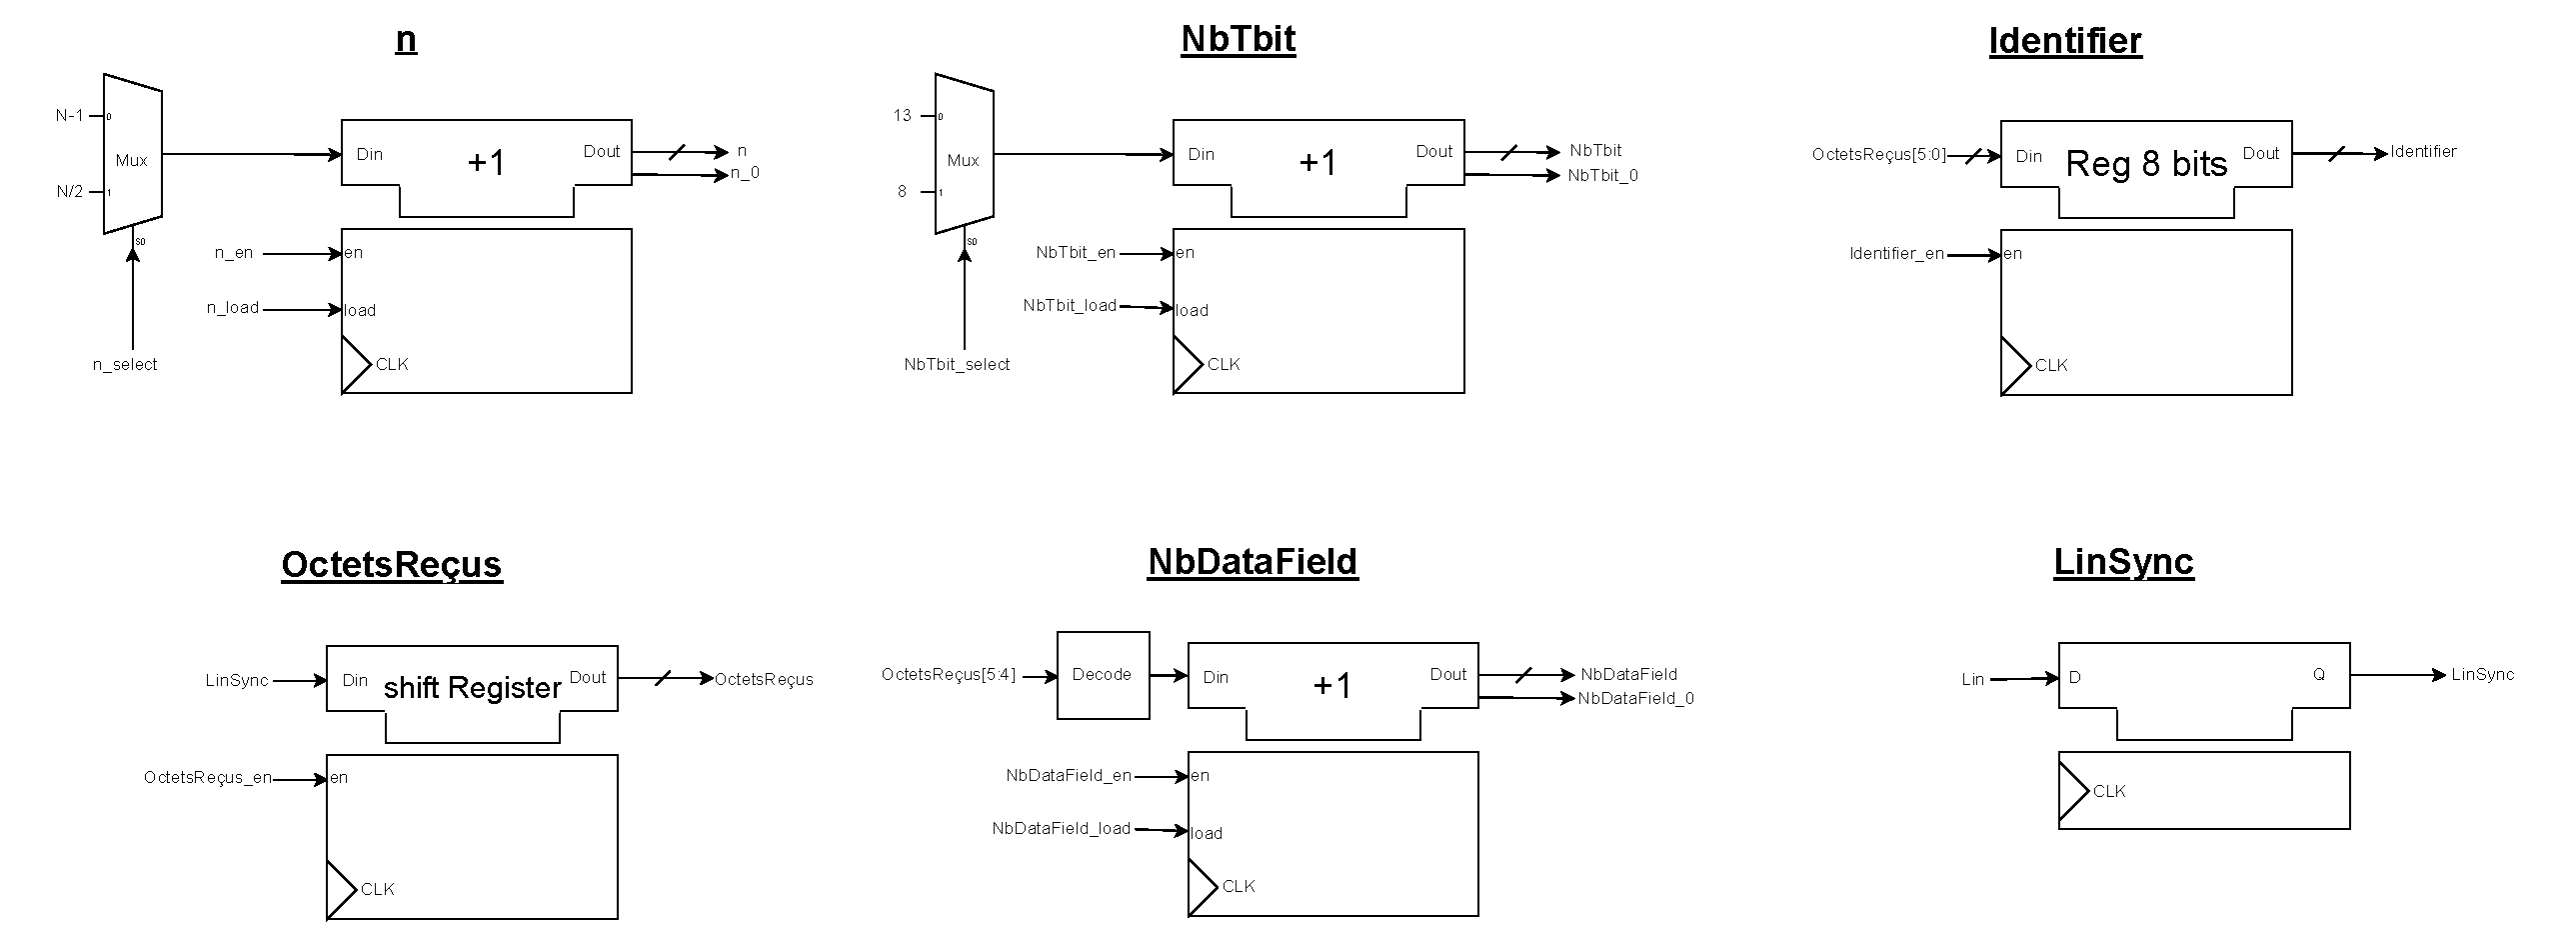
\includegraphics[width=0.95\linewidth]{images/inter/Structure_Reception_trame.pdf}
    \caption{Structure partie Opérative Reception Trame}
    \label{fig:placeholder}
\end{figure}

Dans cette partie nous retrouvons les différents compteurs et registres nécessaires au fonctionnement de la réception de trame. Pour prendre un exemple le premier en haut a gauche reprensente le décompteur n\_0 qui permet de compter jusqu'à N (2048 dans notre cas) pour l'échantillonnage. Le choix de N-1 ou N/2 dépend de l'utilisation, soit N/2 pour la detection de l'état au milieu de Tbit ou N-1 pour la detection de l'état à la fin de Tbit ( Potentiel Front ).
\newline

Pour la partie commande, nous avons conçu et implémenté un automate afin de gérer les différentes séquences de contrôle : 
\newline

%page 21 & 22 TD DAVY 
\begin{figure}[H]
    \centering
    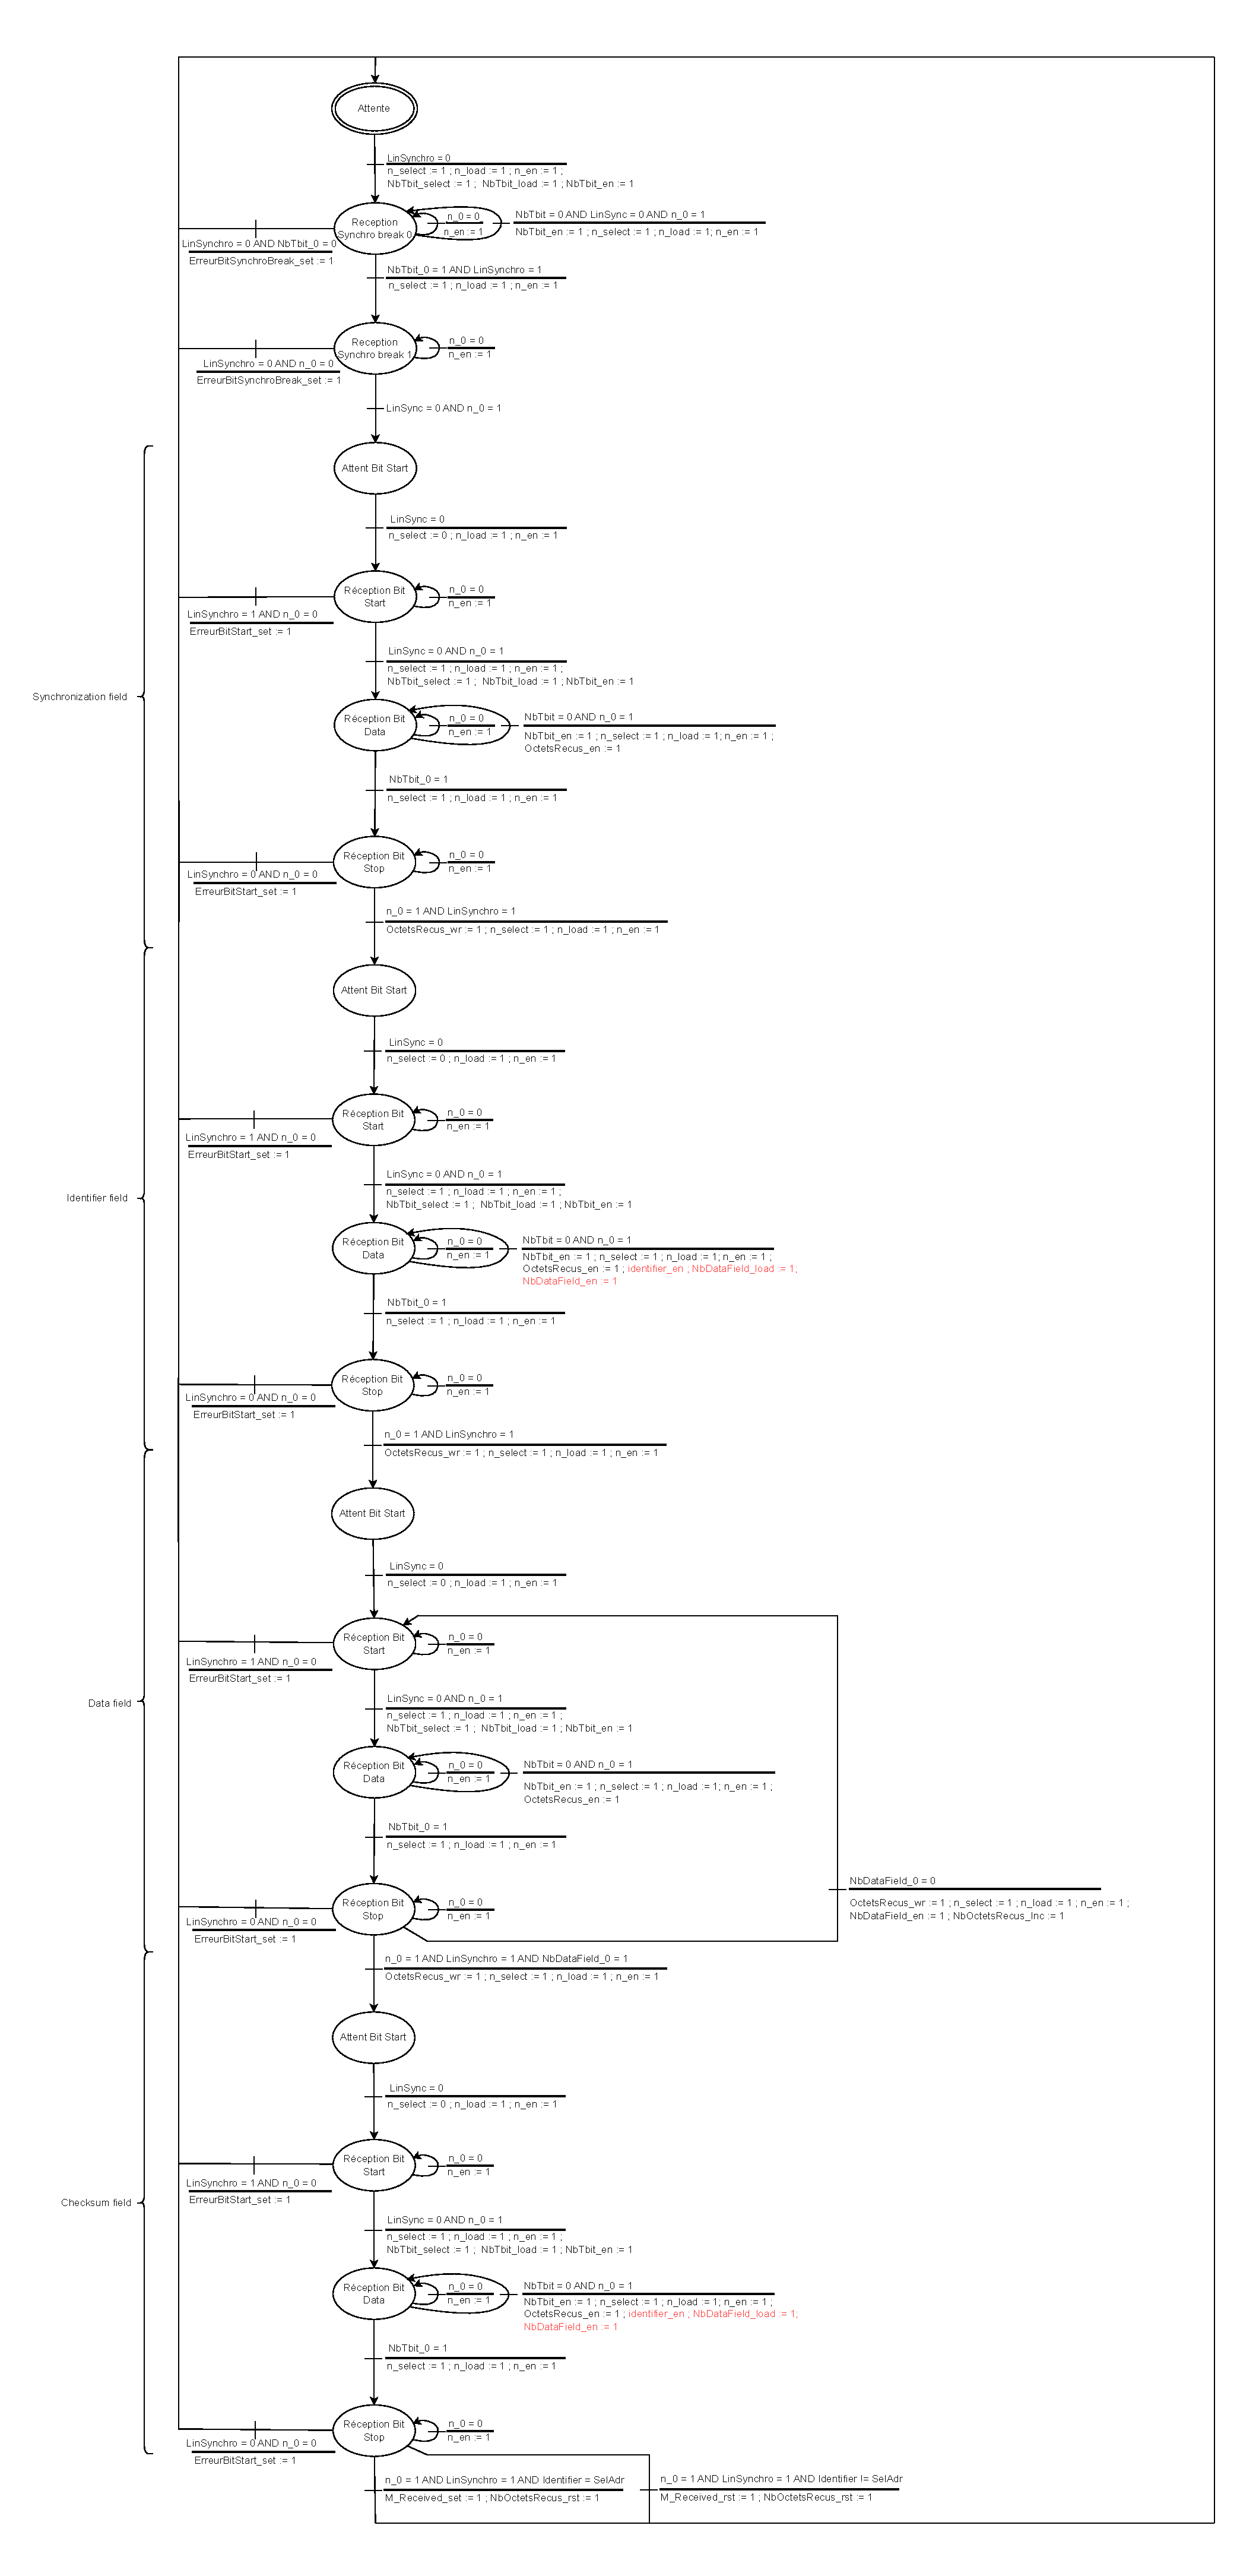
\includegraphics[width=0.6\linewidth]{images/inter/Automate_Reception_trame.pdf}
    \caption{Structure partie Commande Reception Trame}
    \label{fig:placeholder}
\end{figure}

\subsection*{Description de l'automate}
Cet automate décrit un processus de réception de trame LIN (Local Interconnect Network), organisé en états et transitions conditionnées par des signaux de synchronisation, des compteurs et des champs de données. Il commence par une phase d’\textbf{attente}, suivie d’une \textbf{synchronisation sur break} où la ligne (LinSynchro) est surveillée pour détecter le début de la trame. Des erreurs de synchro ou de bit de start peuvent être signalées via des flags comme \texttt{ErreurBitSynchroBreak\_set} ou \texttt{ErreurBitStart\_set}.

Ensuite, l’automate passe à la réception des différents champs de la trame :
\begin{itemize}
    \item \textbf{Synchro} (octet de synchronisation),
    \item \textbf{Identifier} (champ d’identifiant),
    \item \textbf{Data field} (données, avec gestion du compteur \texttt{NbDataField}),
    \item \textbf{Checksum} (vérification de l’intégrité).
\end{itemize}

À chaque octet, le système contrôle le bit de start, les données, et le bit de stop, en incrémentant les compteurs comme \texttt{NbTbit} ou \texttt{NbOctetsRecus}. Selon que l’identifiant reçu correspond ou non à l’adresse sélectionnée (\texttt{SelAdr}), l’automate valide la trame (\texttt{M\_Received\_set}) ou la rejette. Des réinitialisations (\texttt{rst}) ont lieu après réception complète ou en cas d’erreur.

Ce processus assure une réception séquentielle et robuste, typique des protocoles série, avec gestion d’erreurs et validation conditionnelle des trames.

Cet automate peut être représenté sous forme de machine de Mealy, ce qui simplifie l’écriture du code VHDL : 

%page 25 TD DAVY
\begin{figure}[H]
    \centering
    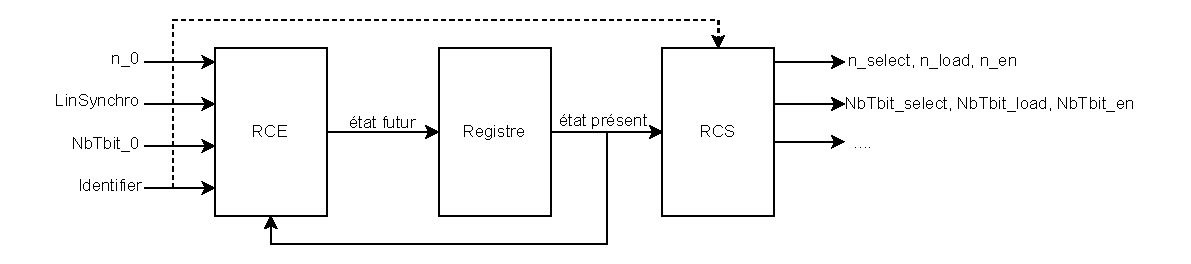
\includegraphics[width=0.8\linewidth]{images/inter/MEALY_Reception_trame.pdf}
    \caption{Machine de MEALY Unité de Commande Reception Trame}
    \label{fig:placeholder}
\end{figure}

\subsection{Architecture Interface MicroProcesseur}

Pour rappel voici tous les signaux associés à ce bloc : 
\newline

\begin{center}
\renewcommand{\arraystretch}{1.2} % espace vertical
\small % pour uniformiser la taille du texte
    \begin{tabularx}{\textwidth}{|c||c|c|X|}
     \hline		
       \textbf{Signaux} & \textbf{Mode} & \textbf{Type} & \textbf{Description}  \\ \hline 
       D07 & INOUT & \texttt{STD\_LOGIC\_VECTOR(7 DOWNTO 0)} & Bus de données \\
       nCS & IN & \texttt{STD\_LOGIC} & Chip Select \\
       RnW & IN & \texttt{STD\_LOGIC} & Opération Lecture / Écriture \\
       CnD & IN & \texttt{STD\_LOGIC} & Opération Contrôle / Données \\
       nCLR & IN & \texttt{STD\_LOGIC} & Réinitialisation \\
       M\_Received & OUT & \texttt{STD\_LOGIC} & Fin de réception de la trame \\
       H & IN & \texttt{STD\_LOGIC} & Horloge \\
       EtatLu & IN & \texttt{STD\_LOGIC\_VECTOR(3 DOWNTO 0)} & Octet d'information de la Trame \\
       DecNbOctet & OUT & \texttt{STD\_LOGIC} & Flag de lecture pour FIFO \\
       EtatLu\_RST & OUT & \texttt{STD\_LOGIC} & Reset de l'état lu \\
       OctetLu & IN & \texttt{STD\_LOGIC\_VECTOR(7 DOWNTO 0)} & Bus de données de sortie \\
       OctetLu\_RD & OUT & \texttt{STD\_LOGIC} & Sélection de la mémoire (Control / Data) \\
     \hline  
    \end{tabularx}
\end{center}

Pour le bloc d'interface Microprocesseur, nous implémentons une machine séquentielle qui permet de distinguer une partie opérative et une partie commande, assurant ainsi la gestion efficace du controle du systeme et la lecture des différentes informations.

%page 24 BAS TD DAVY schema bas
\begin{figure}[H]
    \centering
    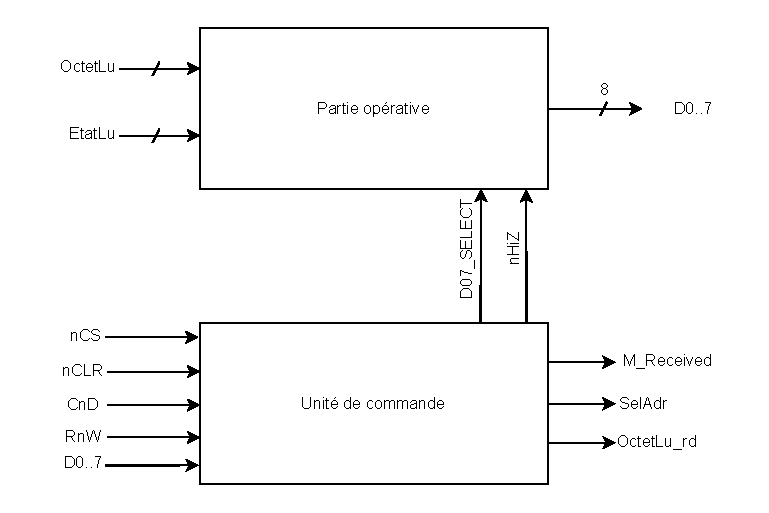
\includegraphics[width=0.8\linewidth]{images/inter/Machine_Seq_Interface_Micro.pdf}
    \caption{Machine Sequentielle Reception Trame}
    \label{fig:placeholder}
\end{figure}

% Page 24 shema haut 
\begin{figure}[H]
    \centering
    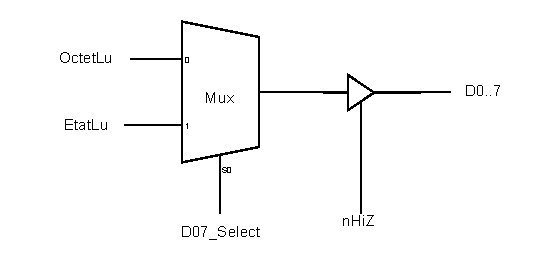
\includegraphics[width=0.8\linewidth]{images/inter/Structure_Interface_Micro.pdf}
    \caption{Structure partie Opérative Interface Microprocesseur}
    \label{fig:placeholder}
\end{figure}

Pour la partie opérative de l’interface microprocesseur, nous obtenons un schéma simple de multiplexeur permettant de choisir quelles données mettre dans le vecteur D07 en sortie, soit celles provenant de la FIFO, soit celles de l’État interne.
\newline

Pour la partie commande, nous avons conçu et implémenté un automate afin de gérer les différentes séquences de contrôle : 
\newline


\begin{figure}[H]
    \centering
    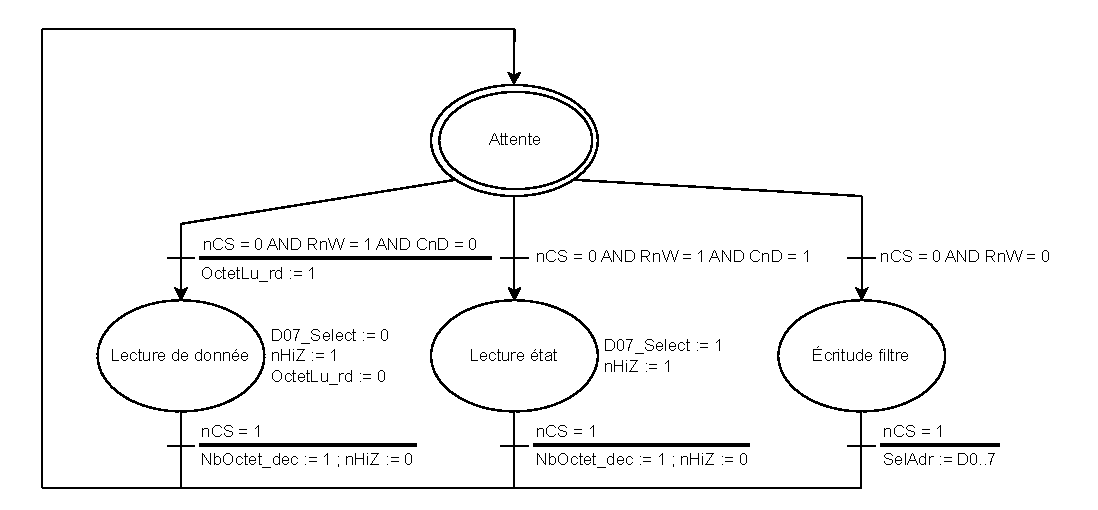
\includegraphics[width=0.8\linewidth]{images/inter/Automate_Interface_Micro.pdf}
    \caption{Structure partie Commande Interface Microprocesseur}
    \label{fig:placeholder}
\end{figure}

Cet automate peut être représenté sous forme de machine de Mealy, ce qui simplifie l’écriture du code VHDL : 

\begin{figure}[H]
    \centering
    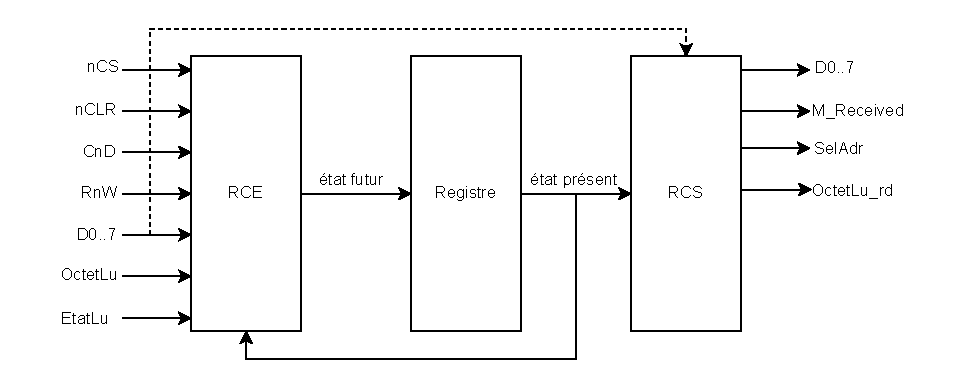
\includegraphics[width=0.8\linewidth]{images/inter/MEALY_Interface_Micro.pdf}
    \caption{Machine de MEALY Unité de Commande Interface Micro}
    \label{fig:placeholder}
\end{figure}

\subsection{Architecture FIFO}

Pour rappel voici tous les signaux associés à ce bloc : 
\newline

\begin{center}
\renewcommand{\arraystretch}{1.2} % espace vertical
\small % pour uniformiser la taille du texte
    \begin{tabularx}{\textwidth}{|c||c|c|X|}
     \hline				
       \textbf{Signaux} & \textbf{Mode} & \textbf{Type} & \textbf{Description}  \\ \hline 
       OctetRecu & IN & \texttt{STD\_LOGIC\_VECTOR(7 DOWNTO 0)} & Bus de données d’entrée \\
       OctetRecu\_WR & IN & \texttt{STD\_LOGIC} & Read / Write opération \\
       OctetRecu\_RST & IN & \texttt{STD\_LOGIC} & Réinitialisation des données reçues \\
       OctetLu & OUT & \texttt{STD\_LOGIC\_VECTOR(7 DOWNTO 0)} & Bus de données de sortie \\
       OctetLu\_RD & IN & \texttt{STD\_LOGIC} & Sélection de la mémoire (Control / Data) \\
     \hline  
    \end{tabularx}
\end{center}

Étant donné que ce système est moins complexe que les deux interfaces précédentes, nous avons choisi de ne pas le réaliser sous forme de machine séquentielle et de le représenter directement comme un bloc, comme montré ci-dessous : 
\newline

%page 14 haut
\begin{figure}[H]
    \centering
    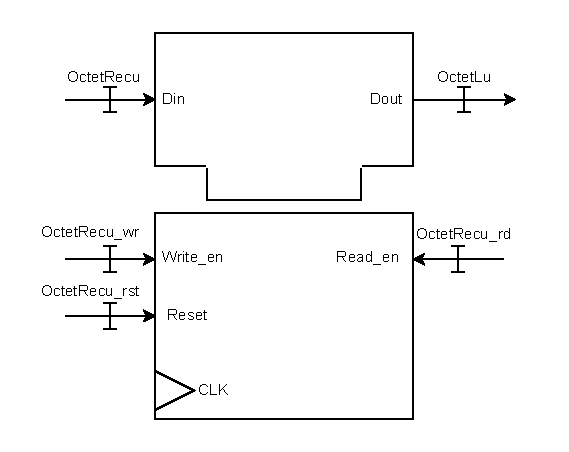
\includegraphics[width=0.8\linewidth]{images/inter/Implementation_FIFO.pdf}
    \caption{Implémentation de la FIFO}
    \label{fig:placeholder}
\end{figure}

\subsection{Implémentation de l’État Interne}

Pour rappel voici tous les signaux associés à ce bloc : 
\newline

\begin{center}
\renewcommand{\arraystretch}{1.2} % espace vertical
\small % pour uniformiser la taille du texte
    \begin{tabularx}{\textwidth}{|c||c|c|X|}
     \hline				
       \textbf{Signaux} & \textbf{Mode} & \textbf{Type} & \textbf{Description}  \\ \hline 
       Erreur\_Start & IN & \texttt{STD\_LOGIC} & Bit d’erreur de Start \\
       Erreur\_Stop & IN & \texttt{STD\_LOGIC} & Bit d’erreur de Stop\\
       Erreur\_SynchroBreak & IN & \texttt{STD\_LOGIC} & Bit d’erreur de Synchro Break\\
       IncNbOctet & IN & \texttt{STD\_LOGIC} & Flag de reception pour lecture \\
       MessageReceived\_SET & IN & \texttt{STD\_LOGIC} & Indicateur de trame reçue \\
       NbOctetRecu\_RST & IN & \texttt{STD\_LOGIC} & Réinitialisation du compteur d’octets \\
       EtatLu & OUT & \texttt{STD\_LOGIC\_VECTOR(7 DOWNTO 0)} & Octet d'information de la Trame \\
       DecNbOctet & IN & \texttt{STD\_LOGIC} & Flag de lecture pour FIFO \\
       EtatLu\_RST & IN & \texttt{STD\_LOGIC} & Reset de l'état lu \\
     \hline  
    \end{tabularx}
\end{center}

Étant donné que ce système présente une complexité similaire et une facilité d’implémentation comparable, nous le conservons également sous forme de bloc, comme montré ci-dessous : 
\newline

%page 14 bas
\begin{figure}[htbp]
    \centering
    \begin{subfigure}[b]{0.49\textwidth}
        \centering
        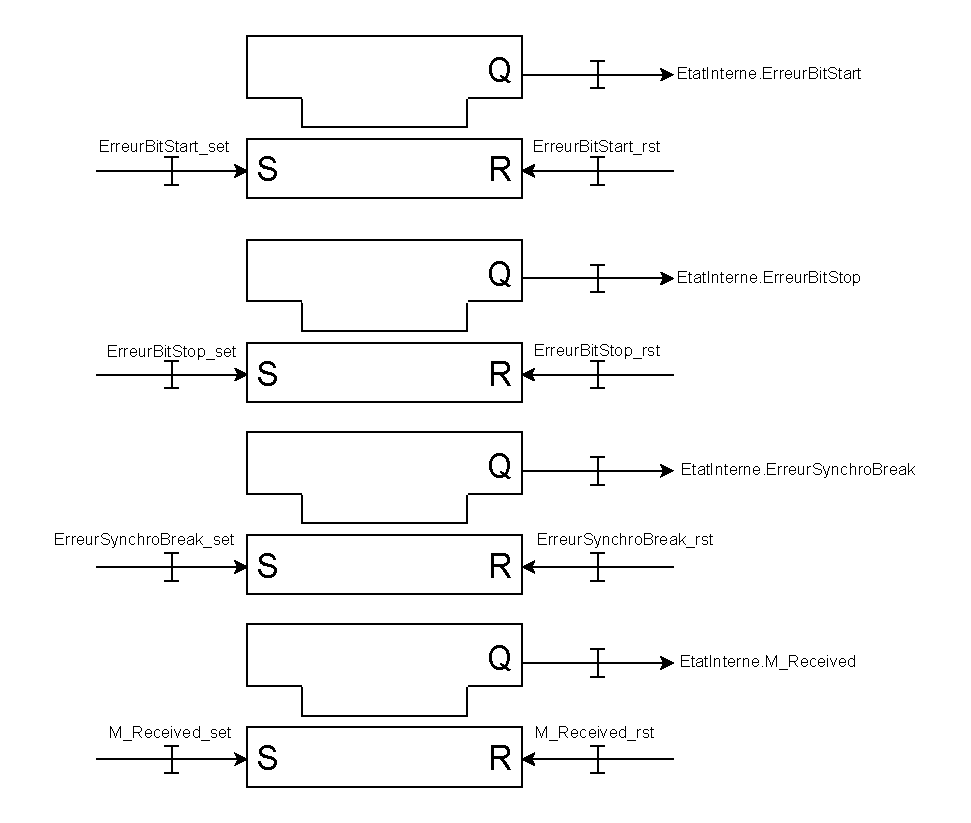
\includegraphics[width=\textwidth]{images/inter/Implementation_ETAT_Erreur.pdf}
        \caption{Mémorisation de l'erreur}
        \label{fig:placeholder}
    \end{subfigure}
    \hfill
    \begin{subfigure}[b]{0.49\textwidth}
        \centering
        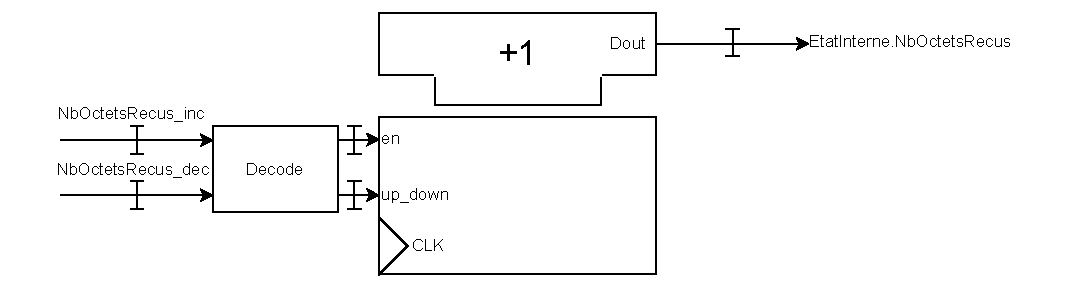
\includegraphics[width=\textwidth]{images/inter/Implementation_ETAT_NbOctets.pdf}
        \caption{Nombre d'octets reçus}
        \label{fig:placeholder}
    \end{subfigure}
    \caption{implémentation de l'état interne en représentation structurelle au niveau RT}
    \label{fig:placeholder} % This is the label for the global figure
\end{figure}
